\section{Theorie}
\label{sec:Theorie}

Die Theorie wird in drei Abschnitte gegliedert: Zum Einen in den Begriff der Interferenz und
die Voraussetzungen für Interferenzeffekte, weiterhin in die Interferenzeffekte mit
kohärentem Licht und zuletzt in die Theorie des Michelson-Interferometers.


\subsection{Interferenz}
\label{sec:interferenz}

\subsubsection{Der Begriff der Interferenz}
\label{sec:interferenzdef}
Die Interferenz beschreibt das Phänomen, das auftritt, wenn Wellen -- hier Licht als
elektromagnetische Welle -- überlagert werden.
Die Intensitäten der Wellen werden nicht nur addiert, sondern zusätzlich mit einem
Interferenzterm multipliziert. Daher können sich Wellen verstärken, was \textbf{konstruktive
Interferenz} genannt wird und gegenseitig auslöschen (\textbf{destruktive Interferenz}).

Die Lichtausbreitung im Vakuum lässt sich durch ebene elektromagnetische Wellen
\begin{equation}
	\label{eqn:ebenewelle}
	\vec{E}(x,t) = \vec{E}_0 \cos(k x - \omega t - \delta)
\end{equation}
beschreiben, wobei $\vec{E}$ der elektrischen Feldstärke, $x$ dem Ort, $t$ der Zeit, $k=\frac{2\pi}{\lambda}$ der Wellenzahl, $\lambda$
der Wellenlänge, $\omega$ der Kreisfrequenz und $\delta$ dem Phasenunterschied bezüglich eines
festen Bezugspunktes entspricht.\\
Die Beschreibbarkeit der Ausbreitung des Lichts durch elektromagnetische Wellen impliziert die
Gültigkeit der Maxwell'schen Gleichungen. Diese sind lineare Differentialgleichungen. Daher
gilt das Prinzip der linearen Superposition, welches besagt, dass ein elektrisches Feld
$\vec{E}$, das aus mehreren einzelnen elektrischen Feldern $\vec{E}_{\mathrm{i}}$
zusammengesetzt wird, der Summe dieser, also $\vec{E} = \sum \vec{E}_{\mathrm{i}}$, entspricht.

Weiterhin ist die Feldstärke von Licht, aufgrund der hohen Frequenz, von
Messgeräten nicht messbar. Daher wird die Intensität von Licht, die Lichtleistung pro
Fläche, betrachtet.
Aus den Maxwell'schen Gleichungen ergibt sich diese zu
\begin{equation}
	\label{eqn:intensity}
	I = C \cdot |\vec{E}|^2 \mathrm{, } \, C = \mathrm{const.}
\end{equation}
Mit den Gleichungen \eqref{eqn:ebenewelle} und \eqref{eqn:intensity} und der linearen
Superposition ergibt sich für die Gesamtintensität $I_{\mathrm{GES}}$ von zwei Lichtwellen mit
der gleichen Amplitude $\vec{E}_0$, die an einem festen Ort $x$ einfallen,
\begin{equation}
	I_{\mathrm{GES}} = \frac{C}{t_2 - t_1} \int_{t_1}^{t_2} |\vec{E_1} + \vec{E_2}|^2(x,t) \,  \symup{d}t \mathrm{,}
\end{equation}
wobei das Beobachtungsintervall $t_2 - t_1$ groß gegen die Periodendauer $T=\frac{2\pi}{\omega}$
sein soll.
Einsetzen und Ausmultiplizieren liefert schließlich
\begin{equation}
	\label{eqn:4}
	I_{\mathrm{GES}} = 2C \, \vec{E_0}^2 (1+\cos(\delta_2 - \delta_1)) \mathrm{,}
\end{equation}
den Interferenzterm. Die Intensitäten weichen bei einem Phasenunterschied von
$\delta_2 - \delta_1 = n \cdot 2\pi$ um $2C \vec{E_0}^2$ vom Mittelwert ab und verschwinden
bei einem Phasenunterschied von $(2n+1) \cdot \pi$, mit $n \in \mathbb{N}$.


\subsubsection{Diskussion über die Voraussetzungen zur Messung von Interferenzerscheinungen}
\label{sec:messunginterferenz}

Werden Lichtwellen aus verschiedenen Quellen überlagert, sind keine Interferenzeffekte zu
beobachten. Dies hat die Ursache, dass bei der Emission von Lichtwellen Elektronen
Emissionszentren darstellen: Die Elektronen werden durch hinzugefügte Energie in einen
angeregten Zustand versetzt und emittieren bei der Rückkehr in den Grundzustand Energie in Form
eines Wellenzuges endlicher Länge, also einer Wellengruppe. \\Des Weiteren treten diese Emissionen
statistisch verteilt in der Elektronenhülle des Atoms bzw. Moleküls auf und daher sind die Phasen
$\delta_1$ bzw. $\delta_2$ statistische Funktionen der Zeit.

Daraus folgt, dass die Mittelung über die Zeit
\begin{equation}
	\frac{1}{t_2-t_1} \int_{t_1}^{t_2} C \, \cos(\delta_2(t)-\delta_1(t)) \, \symup{d}t
\end{equation}
verschwindet, da das Beobachtungsintervall $t_2-t_1$ groß gegen die Periodendauer $T$ ist und
der Phasenunterschied $\delta_2-\delta_1$ beliebige Werte annimmt.

Licht aus verschiedenen Quellen ist also nicht interferenzfähig, es ist \textbf{inkohärent}.
Interferenzeffekte lassen sich also nur erzeugen, wenn das Licht aus der selben Quelle stammt,
sogenanntes \textbf{kohährentes} Licht.


\subsection{Interferenzeffekte mit kohärentem Licht}
\label{sec:kohärenz}

Um Interferenzeffekte mit kohärentem Licht erzeugen zu können, muss die Quelle Licht mit
festem $k$, $\omega$ und $\delta$ (vergleiche Gleichung \eqref{eqn:ebenewelle}) emittieren.\\
Weiterhin muss der Strahlengang des Lichtes getrennt werden, damit sich die beiden Teilwellen
an einem Punkt P überlagern können.\\
Der Unterschied der Weglängen der beiden Teilwellen wird \textbf{Wegunterschied $\Delta$}
genannt.
Hierbei ist zu beachten, dass der Wegunterschied $\Delta$ nicht zu groß gegen die Länge eines
Wellenzugs sein darf. Dies liegt daran, dass ein Emissionsakt eine endliche Dauer $\tau$ und der
emittierte Wellenzug somit eine endliche Länge hat. Ist der Wegunterschied $\Delta$ zu groß
gegen die Länge dieses Wellenzuges, treffen Teilwellen aus unterschiedlichen Wellenzügen
zeitgleich am Punkt P auf und können aufgrund der inkonstanten Phasenbeziehung zueinander nicht
interferieren.
Der Wegunterschied $\Delta$, ab dem keine Interferenzeffekte auftreten, heißt \textbf{Kohärenzlänge $\ell$}.\\ Sie ergibt sich aus der Anzahl $N$ der im Interferenzbild
auftretenden Intensitätsmaxima und der Wellenlänge $\lambda$ zu
\begin{equation}
	\ell = N \lambda \, \mathrm{.}
\end{equation}
Außerdem ergibt sich aus dem \textbf{Fourier'schem Theorem}, dass ein Wellenzug endlicher
Länge nicht monochromatisch ist und ein Frequenz- und Wellenlängenspektrum hat. Dieses
Spektrum sorgt für ein unklares Interferenzbild, weil eine Frequenz aus dem Spektrum in einem
Punkt bei einem gewissen Wegunterschied $\Delta$ ein Maximum haben kann, während eine andere
Frequenz aus dem Spektrum destruktiv interferiert. Daher muss entweder das Spektrum oder der
Wegunterschied sehr klein sein, damit sich Maxima und Minima nicht in einem Punkt überschneiden.

Das Frequenzspektrum eines Wellenzuges ergibt sich durch eine Fourier-Transformation der
Feldstärke zu
\begin{equation}
	g(\omega) = 2E_0 \frac{\sin{(\omega-\omega_0)\cdot\frac{\tau}{2}}}{\omega-\omega_0}
\end{equation}
und damit die Intensität als Betragsquadrat zu
\begin{equation}
	\label{eqn:waveintensity}
	G(\omega) = |g(\omega)|^2 = 4E_0^2 \frac{\sin^2(\omega-\omega_0)\frac{\tau}{2}}{(\omega- \omega_0)^2} \mathrm{.}
\end{equation}
Die Intensitätsverteilung \eqref{eqn:waveintensity} hat ein Maximum bei $\omega=\omega_0$ und
als Verteilungsfunktion die Breite $\Delta \omega = \frac{2\pi}{\tau}$.
Mit dem Zusammenhang
\begin{equation}
	\lambda_0 := \frac{2\pi \symup{c}}{\omega_0} \mathrm{,}
\end{equation}
der Breite $\Delta \omega = \frac{2\pi}{\tau}$ der Verteilungsfunktion $G(\omega)$ und
Differentiation ergibt sich
\begin{equation}
	\Delta \lambda = \frac{\lambda_0^2}{\symup{c}\tau}
\end{equation}
und wegen der Dauer eines Wellenzuges $\tau = \frac{\ell}{\symup{c}}$
(auch \textbf{Kohärenzzeit}) ein Zusammenhang zwischen der Kohärenzlänge $\ell$, der Dauer
eines Wellenzuges $\tau$ und der Breite $\Delta \lambda$ der Wellenlängen- und Frequenzverteilung zu
\begin{equation}
	\Delta \lambda = \frac{\lambda_0^2}{\ell} \mathrm{.}
\end{equation}
\begin{figure}
	\caption{Versuchsanordnung zur Kohärenzbedingung ausgedehnter Lichtquellen}
	\label{fig:...}
	\centering
	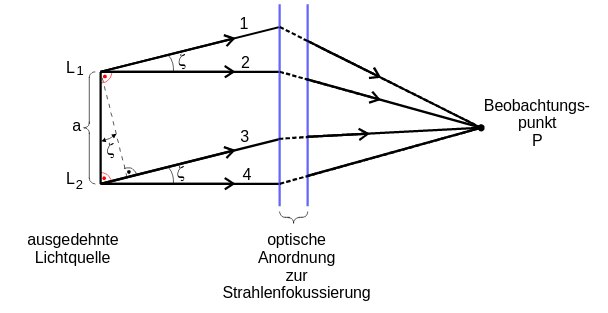
\includegraphics[width=0.85\textwidth]{Bilder/ausgedehnte_lichtquelle.png}
\end{figure}
Des Weiteren zu beachten ist, dass in der Realität verwendete Lichtquellen nicht punktförmig
sind, sondern eine endliche Ausdehnung haben. Strahlen, die von einer ausgedehnten Lichtquelle
(siehe Abbildung \ref{fig:...}) aus durch eine Linse auf einen Beobachtungspunkt P fokussiert
werden, können paarweise interferieren, wenn sie aus dem gleichen Punkt emittiert wurden.\\
Durch den Winkel $\zeta$ in Abbildung \ref{fig:...} tritt eine zusätzliche Phasenverschiebung
$\Delta \phi$ zwischen den Strahlen 3 und 4 auf, sodass das Interferenzbild im Punkt P
zerstört werden kann, wenn die Phasenverschiebung $\Delta \phi$ durch den Winkel $\zeta$ nicht
viel kleiner als $\pi$ ist.
\\Somit ergibt sich mit
\begin{equation}
	\Delta \phi = \frac{2\pi}{\lambda} a \sin(\zeta) \mathrm{,}
\end{equation}
die \textbf{Kohärenzbedingung für ausgedehnte Lichtquellen} zu
\begin{equation}
	a \sin(\zeta) \ll \frac{\lambda}{2} \mathrm{.}
\end{equation}


\subsection{Die Theorie des Michelson-Interferometers}

Das Michelson-Interferometer erlaubt, mithilfe der Betrachtung von Interferenzeffekten, die Messung optischer Größen.
Um Interferenzen zu erhalten, ist es nötig, einen Lichtstrahl in zwei Teilbündel zu zerteilen und diese, nachdem ein Teilbündel beispielsweise einer Variation seines optischen Wegs erfahren hat, wieder zusammenzuführen.\\
Beim Michelson-Morley Experiment erfolgt die Strahlteilung mittels einer semipermeablen Platte $P$ .
Eines der Strahlbündel geht dabei ohne Richtungsänderung durch den Strahlteiler zu Spiegel $S_2$, der Rest wird senkrecht zum ursprünglichen Strahl hin zu Spiegel $S_1$ gebrochen.\\
Beide Strahlbündel werden an den Spiegeln reflektiert und treffen am Strahlteiler $P$ wieder zusammen. Jeweils ein Teil der Strahlbündel läuft nun zurück zur Quelle $L$ und wird auch nicht weiter betrachtet. Die anderen Teile der beiden Strahlbündel laufen parallel zum Beobachtungsort $D$.\\
Sofern der optische Wegunterschied der beiden Strahlbündel kleiner ist als die Kohärenzlänge der Lichtquelle, sind die am Beobachtungsort ankommenden Strahlbündel kohärent.\\
Im Strahlweg des Strahlbündels $S_2$ wird eine zusätzliche Kompensationsplatte eingebracht, da das Strahlbündel $S_1$ dreimal die semipermeable Platte passiert, während selbige durch das Strahlbündel $S_2$ nur einmal passiert wird.\\
Sind beide Strahlwege exakt gleich lang realisiert, kommt es dennoch am Beobachtungsort $D$ zur destruktiven Interferenz, da das Strahlbündel $S_2$ bei der Reflexion am Strahlteiler einen Phasensprung erfährt.\\
Wird einer der Spiegel um das Wegstück $\Delta d$ verschoben, besteht ein Wegunterschied von $2\Delta d$ zwischen beiden Strahlwegen.
Mit den bereits angestellten Überlegungen wird nach Formel \eqref{eqn:4} folglich also die Intensität am Beobachtungsort immer zwischen 0 und einem Maximalwert schwanken.
Werden die Intensitätsmaxima pro Verschiebestrecke $\Delta d$ gezählt, ergibt sich die Wellenlänge zu:
\begin{equation}
	\label{eqn:lambda}
	\lambda= \Delta\text{d}\cdot \frac{2}{z} \text{.}
\end{equation}
Eine Variation der optischen Weglänge lässt sich außerdem erreichen, indem eines der Teilbündel beispielsweise durch eine Messzelle mit einem Medium mit geänderten Brechungsindex läuft.\\
Das Michelson-Interferometer kann damit auch zur Bestimmung des Brechungsindex eines Gases verwendet werden.
Dazu wird die Messzelle bestmöglichst auf den Druck $p'$ evakuiert und das zu untersuchende Gas wird in die Messzelle strömen gelassen, bis wieder der Umgebungsdruck $p$ erreicht ist.
In der Messzelle herrsche der Brechungsindex $n+ \Delta n$. Der Umgebungsdruck sei $n$.
\\Der optische Wegunterschied zwischen beiden Strahlwegen beträgt $b\cdot \Delta d$. Hierbei ist $b$ die Breite der Messzelle.
\\Die Anzahl $z$ der gezählten Intensitätsmaxima am Beobachtungsort multipliziert mit der halben Wellenlänge ist gleich dem optischen Wegunterschied.
\\Die Differenz des Brechungsindex bestimmt sich daher nach
\begin{equation}
\label{eqn:deltan}
\Delta n= \frac{z \lambda}{2b} \text{.}
\end{equation}
Der Brechungsindex unter Normalbedingungen eines zu untersuchenden Gases in der Messzelle ergibt sich mit der Dispersionstheorie und der Idealen Gasgleichung zu
\begin{equation}
\label{eqn:n}
	n(p_0,T_0)=1+\Delta n \cdot \frac{T}{T_0}\frac{p_0}{\Delta p} \text{.}
\end{equation}
Hierbei ist $T$ die Umgebungstemperatur, $\Delta p$ die Druckdifferenz $p-p'$ und $\Delta n$ ergibt sich nach Formel \eqref{eqn:n}.
